\chapter{Designing Classes}

\index{object!type}
\index{type!object}

Whenever you create a new class, you are creating a new object type with the same name.
So way back in Section~\ref{hello}, when we created the class \java{Hello}, we also created an object type named \java{Hello}.

We didn't declare any variables with type \java{Hello}, and we didn't use \java{new} to create \java{Hello} objects.
And it wouldn't have done much good if we had -- but we could have!

In this chapter, you will learn to design classes that represent {\em useful} objects.  Here are the main ideas:

\begin{itemize}

\item Again, defining a {\bf class} creates a new object type with the same name.

\index{class!definition}

\item A class definition is a template for objects: it specifies what attributes the objects have and what methods can operate on them.

\index{instance}

\item Every object belongs to some object type; that is, it is an {\bf instance} of some class.

\index{instantiate}

\item The \java{new} operator {\bf instantiates} objects; that is, it creates new instances of a class.

%\item The design of a class (what methods it has) determines whether the objects are mutable or immutable.

% \item The methods that operate on an object type are defined in the class for that object.

\end{itemize}

Think of a class like a blueprint for a house: you can use the same blueprint to build any number of houses.

\section{The Time Class}

%\index{data encapsulation}
%\index{encapsulation!data}

A common reason to define a new class is to encapsulate related data in an object that can be treated as a single unit.
That way, we can use objects as parameters and return values, rather than passing and returning multiple values.
%This design principle is called {\bf data encapsulation}.
We have already seen two types that encapsulate data in this way: \java{Point} and \java{Rectangle}.

\index{class!Time}
\index{Time}

Another example, which we will implement ourselves, is \java{Time}, which represents a time of day.
The data encapsulated in a \java{Time} object include an hour, a minute, and a number of seconds.
Because every \java{Time} object contains these values, we define attributes to hold them.

\index{instance variable}
\index{variable!instance}

Attributes are also called {\bf instance variables}, because each instance has its own variables (as opposed to ``class variables'', coming up in Section~\ref{classvar}).

The first step is to decide what type each variable should be.
It seems clear that \java{hour} and \java{minute} should be integers.
Just to keep things interesting, let's make \java{second} a double.

Instance variables are declared at the beginning of the class definition, outside of any method.
By itself, this code fragment is a legal class definition:

\begin{code}
public class Time {
    private int hour;
    private int minute;
    private double second;
}
\end{code}

\index{private}
\index{variable!private}

The \java{Time} class is \java{public}, which means that it can be used in other classes.
But the instance variables are \java{private}, which means they can only be accessed from inside the \java{Time} class.
If you try to read or write them from another class, you will get a compiler error.

\index{information hiding}

Private instance variables help keep classes isolated from each other, so that changes in one class won't require changes in other classes.
It also simplifies what other programmers need to know to use your classes.
This kind of isolation is called {\bf information hiding}.


\section{Constructors}

\index{constructor}
\index{method!constructor}

After declaring instance variables, the next step is to define a {\bf constructor}, which is a special method that initializes the object.
The syntax for constructors is similar to that of other methods, except:

\index{static}

\begin{itemize}

\item The name of the constructor is the same as the name of the class.

\item Constructors have no return type (and no return value).

\item The keyword \java{static} is omitted.

\end{itemize}

Here is an example constructor for the \java{Time} class:

\begin{code}
public Time() {
    this.hour = 0;
    this.minute = 0;
    this.second = 0.0;
}
\end{code}

This constructor does not take any arguments.
Each line initializes an instance variable to zero (which is ``midnight'' for a \java{Time} object).

\index{this}
\index{keyword}

The name \java{this} is a keyword that refers to the object we are creating.
You can use \java{this} the same way you use the name of any other object.
For example, you can read and write the instance variables of \java{this}, and you can pass \java{this} as an argument to other methods.
But you do not declare \java{this}, and you can't make an assignment to it.

A common error when writing constructors is to put a \java{return} statement at the end.
Like \java{void} methods, constructors do not return values.

To create a \java{Time} object, you must use the \java{new} operator:

\begin{code}
public static void main(String[] args) {
    Time time = new Time();
}
\end{code}

\index{new}
\index{operator!new}

When you use \java{new}, Java creates the object and invokes your constructor to initialize the instance variables.
When the constructor is done, \java{new} returns a reference to the new object.
In this example, the reference gets assigned to the variable \java{time}, which has type \java{Time}.
Figure~\ref{fig.time} shows the result.

\index{memory diagram}
\index{diagram!memory}

\begin{figure}[!ht]
\begin{center}
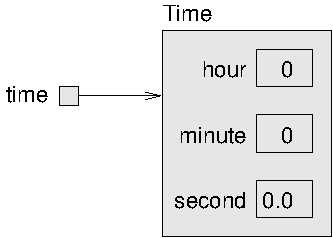
\includegraphics{figs/time.pdf}
\caption{Memory diagram of a \java{Time} object.}
\label{fig.time}
\end{center}
\end{figure}

\index{recursion!infinite}
\index{infinite recursion}
\index{StackOverflowError}

Beginners sometimes make the mistake of using \java{new} in the constructor:

\begin{code}
public Time() {
    new Time();         // StackOverflowError
    this.hour = 0;
    this.minute = 0;
    this.second = 0.0;
}
\end{code}

Doing so causes an infinite recursion, since \java{new} invokes the {\em same} constructor, which uses \java{new} again, which invokes the constructor again, and so on.

%If you don't provide a constructor for a class, Java will generate one for you automatically.
%The default constructor takes no arguments and initializes all attributes to zero (or an equivalent value like \java{false} or \java{null}).


\section{Value Constructors}

\index{overload}

Like other methods, constructors can be overloaded, which means you can provide multiple constructors with different parameters.
Java knows which constructor to invoke by matching the arguments you provide with the parameters of the constructor.

\index{value constructor}
\index{constructor!value}

It is common to provide both a ``default constructor'' that takes no arguments, like the previous one, and a ``value constructor'', like this one:

\begin{code}
public Time(int hour, int minute, double second) {
    this.hour = hour;
    this.minute = minute;
    this.second = second;
}
\end{code}

To invoke this constructor, you have to provide arguments to the \java{new} operator.
The following example creates a \java{Time} object that represents a fraction of a second before noon:

\begin{code}
Time time = new Time(11, 59, 59.9);
\end{code}

Overloading constructors provides the flexibility to create an object first and then fill in the attributes, or collect all the information before creating the object itself.

Once you get the hang of it, writing constructors gets boring.
You can write them quickly just by looking at the list of instance variables.
In fact, some IDEs can generate them for you.

Here is the complete class definition so far:

%\index{Time.java}

\begin{code}
public class Time {
    private int hour;
    private int minute;
    private double second;

    public Time() {
        this.hour = 0;
        this.minute = 0;
        this.second = 0.0;
    }

    public Time(int hour, int minute, double second) {
        this.hour = hour;
        this.minute = minute;
        this.second = second;
    }
}
\end{code}

Notice how the second constructor declares the parameters \java{hour}, \java{minute}, and \java{second}.
Java allows you to declare parameters (and local variables) with the same names as instance variables.
They don't have to use the same names, but it's common practice.

\index{shadowing}

The right side of \java{this.hour = hour;} refers to the parameter \java{hour}, since it was declared most recently.
This situation is called {\bf shadowing}, because the parameter ``hides'' the instance variable with the same name.

Java provides the keyword \java{this} so you can access instance variables, regardless of shadowing.
As a result, this constructor copies the values from the parameters to the instance variables.


\section{Getters and Setters}

Recall that the instance variables of \java{Time} are \java{private}.
We can access them from within the \java{Time} class, but if we try to read or write them from another class, the compiler reports an error.

\index{private}
\index{variable!private}

A class that uses objects defined in another class is called a {\bf client}.
For example, here is a new class called \java{TimeClient}.

\index{client}

\begin{code}
public class TimeClient {

    public static void main(String[] args) {
        Time time = new Time(11, 59, 59.9);
        System.out.println(time.hour);      // compiler error
    }
}
\end{code}

If you compile this code, you get an error message like ``hour has private access in Time''.
There are three ways to solve this problem:

\begin{itemize}

\item We could make the instance variables public.

\item We could provide methods to access the instance variables.

\item We could decide that it's not a problem, and refuse to let other classes access the instance variables.

\end{itemize}

The first choice is appealing because it's simple.
But here is the problem: when Class $A$ accesses the instance variables of Class $B$ directly, $A$ becomes dependent on $B$.
If anything in $B$ changes later, it is likely that $A$ will have to change, too.

\index{dependent}
\index{independent}

But if $A$ only uses methods to interact with $B$, $A$ and $B$ are less dependent, which means that we can make changes in $B$ without affecting $A$ (as long as we don't change the method parameters).
So we generally avoid making instance variables public.

The second option is to provide methods that access the instance variables.
For example, we might want the instance variables to be ``read only''; that is, code in other classes should be able to read them but not write them.
We can do that by providing one method for each instance variable:

\begin{code}
public int getHour() {
    return this.hour;
}

public int getMinute() {
    return this.minute;
}

public double getSecond() {
    return this.second;
}
\end{code}

\index{accessor}
\index{method!accessor}
\index{getter}
\index{method!getter}

Methods like these are formally called ``accessors'', but more commonly referred to as {\bf getters}.
By convention, the method that gets a variable named \java{something} is called \java{getSomething}.

We can fix the compiler error in \java{TimeClient} by using the getter:

\begin{code}
System.out.println(time.getHour());
\end{code}

If we decide that \java{TimeClient} should also be able to modify the instance variables of \java{Time}, we can provide methods to do that, too:

\begin{code}
public void setHour(int hour) {
    this.hour = hour;
}

public void setMinute(int minute) {
    this.minute = minute;
}

public void setSecond(double second) {
    this.second = second;
}
\end{code}

\index{mutator}
\index{method!mutator}
\index{setter}
\index{method!setter}

These methods are formally called ``mutators'', but more commonly known as {\bf setters}.
The naming convention is similar; the method that sets \java{something} is usually called \java{setSomething}.

Writing getters and setters can get boring, but many IDEs can generate them for you based on the instance variables.

% NOTE: A thougtful reader might ask a question we don't answer here: if we provide getters and setters, why don't we just make the instance variables public? 


\section{Displaying Objects}

To display \java{Time} objects we can write a method to display the hour, minute, and second.
Using \java{printTime} in Section~\ref{multparam} as a starting point, we could write:

\begin{code}
public static void printTime(Time t) {
    System.out.print(t.hour);
    System.out.print(":");
    System.out.print(t.minute);
    System.out.print(":");
    System.out.println(t.second);
}
\end{code}

The output of this method, given the \java{time} object from the first example, would be {\tt 11:59:59.9}.
We can use \java{printf} to make the code more concise:

\index{printf}
\index{print statement}
\index{format string}

\begin{code}
public static void printTime(Time t) {
    System.out.printf("%02d:%02d:%04.1f\n",
        t.hour, t.minute, t.second);
}
\end{code}

As a reminder, you need to use \java{\%d} with integers and \java{\%f} with floating-point numbers.
The \java{02} option means ``total width 2, with leading zeros if necessary'', and the \java{04.1} option means ``total width 4, one digit after the decimal point, leading zeros if necessary''.
The output is the same: {\tt 11:59:59.9}.

There's nothing wrong with a method like \java{printTime}, but it is not consistent with object-oriented style.
A more idiomatic solution is to provide a special method called \java{toString}.


\section{The toString Method}

Every object has a method called \java{toString} that returns a string representation of the object.
When you display an object using \java{print} or \java{println}, Java invokes the object's \java{toString} method.

\index{override}

By default it simply displays the type of the object and its address in hexadecimal. 
So, if you create a \java{Time} object and display it with \java{println}:

\begin{code}
public static void main(String[] args) {
    Time time = new Time(11, 59, 59.9);
    System.out.println(time);
}
\end{code}

\index{print}
\index{statement!print}
\index{object!displaying}

The output looks something like this:

\begin{stdout}
Time@80cc7c0
\end{stdout}

\index{address}
\index{hexadecimal}

This address can be useful for debugging, if you want to keep track of individual objects.

\index{toString}
\index{method!toString}

But you can {\bf override} this behavior by providing your own \java{toString} method.
For example, here is a \java{toString} method for \java{Time}:

\begin{code}
public String toString() {
    return String.format("%02d:%02d:%04.1f\n",
        this.hour, this.minute, this.second);
}
\end{code}

\index{instance method}
\index{method!instance}

The definition does not have the keyword \java{static}, because it is not a static method.
It is an {\bf instance method}, so called because when you invoke it, you invoke it on an instance of the class.
Instance methods are sometimes called ``non-static''; you might see this term in an error message.

The body of the method is similar to \java{printTime} in the previous section, with two changes:

\begin{itemize}

\item Inside the method, we use \java{this} to refer to the current instance; that is, the object the method is invoked on.

\item Instead of \java{printf}, it uses \java{String.format}, which returns a formatted \java{String} rather than displaying it.

\end{itemize}

\index{string!format}

Now you can call \java{toString} directly:

\begin{code}
Time time = new Time(11, 59, 59.9);
String s = time.toString();
\end{code}

The value of \java{s} is the \java{String} \java{"11:59:59.9"}.

You can also invoke \java{toString} indirectly by invoking \java{print} or \java{println}:

\begin{code}
System.out.println(time);
\end{code}

This code displays the \java{String} \java{"11:59:59.9"}. 

Either way, when you use \java{this} inside \java{toString}, it refers to the same object as \java{time}.


\section{The equals Method}
\label{equals}

\index{== equals operator}
\index{equals}
\index{method!equals}

We have seen two ways to check whether values are equal: the \java{==} operator and the \java{equals} method.
With objects you can use either one, but they are not the same.

\index{identical}
\index{equivalent}

\begin{itemize}

\item The \java{==} operator checks whether two references are {\bf identical}; that is, whether they refer to the same object.

\item The \java{equals} method checks whether two objects are {\bf equivalent}; that is, whether they have the same values.

\end{itemize}

The definition of identity is always the same, so the \java{==} operator always does the same thing.
But the definition of equivalence is different for different objects, so objects can define their own \java{equals} methods.

Consider the following variables and the memory diagram in Figure~\ref{fig.time2}.

\begin{code}
Time time1 = new Time(9, 30, 0.0);
Time time2 = time1;
Time time3 = new Time(9, 30, 0.0);
\end{code}

\index{memory diagram}
\index{diagram!memory}

\begin{figure}[!ht]
\begin{center}
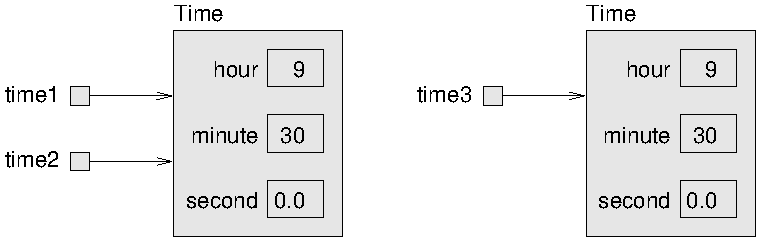
\includegraphics{figs/time2.pdf}
\caption{Memory diagram of three \java{Time} variables.}
\label{fig.time2}
\end{center}
\end{figure}

The assignment operator copies references, so \java{time1} and \java{time2} refer to the same object.
Because they are identical, \java{time1 == time2} is true.
But \java{time1} and \java{time3} refer to two different objects.
Because they are not identical, \java{time1 == time3} is false.

By default, the \java{equals} method does the same thing as \java{==}.
For \java{Time} objects, that's probably not what we want.
For example, \java{time1} and \java{time3} represent the same time of day, so we should consider them equivalent.

\index{equals}
\index{method!equals}

We can provide an \java{equals} method that implements this idea:

\begin{code}
public boolean equals(Time that) {
    final EPS = 0.001;
    return this.hour == that.hour
        && this.minute == that.minute
        && Math.abs(this.second - that.second) < EPS;
}
\end{code}

\java{equals} is an instance method, so it doesn't have the keyword \java{static}.
It uses \java{this} to refer to current object, and \java{that} to refer to the other.
\java{that} is {\em not} a keyword, so we could have given this parameter a different name.
But using \java{that} makes the code nicely readable. 

We can invoke \java{equals} like this:

\begin{code}
time1.equals(time3);
\end{code}

Inside the \java{equals} method, \java{this} refers to the same object as \java{time1}, and \java{that} refers to the same object as \java{time3}.
Since their instance variables are ``equal'', the result is \java{true}.

Because \java{hour} and \java{minute} are integers, we compare them with \java{==}.  
But \java{second} is a floating-point number.  
Because of rounding errors, it is not good to compare floating-point numbers with \java{==} (see Section~\ref{rounderr}).
Instead, we check whether the difference is smaller than a threshold, \java{EPS} (which is short for ``epsilon'', the Greek letter used to represent a small number).

Many objects have a similar notion of equivalence; that is, two objects are considered equal if their instance variables are equal.
But other definitions are possible.


% This example is a little non-idiomatic.  Can we think of something else?

%You could, for example, allow a \java{Time} object and a \java{String} object to be considered equal if they represent the same time.
%
%\begin{code}
%public boolean equals(String str) {
%    return str.equals(this.toString());
%}
%\end{code}
%
%The \java{equals} method is now overloaded.
%If we invoke \java{time1.equals(time3)}, the first method will be used; \java{time1.equals("09:30:00.0")} uses the second.


\section{Adding Times}
\label{addingtime}

Suppose you are going to a movie that starts at 18:50 (that is, 6:50 PM), and the running time is 2 hours 16 minutes.
What time does the movie end?
We'll use \java{Time} objects to figure it out.

\begin{code}
Time startTime = new Time(18, 50, 0.0);
Time runningTime = new Time(2, 16, 0.0);
\end{code}

\index{Time!addition}
\index{addition!time}

Here are two ways we could ``add'' the \java{Time} objects:

\begin{itemize}

\item We could write a static method that takes two \java{Time} objects as parameters.

\item We could write an instance method that gets invoked on one object and takes the other as a parameter.

\end{itemize}

To demonstrate the difference, we'll do both.
Here is the static method:

\index{static}
\index{method!static}

\begin{code}
public static Time add(Time t1, Time t2) {
    Time sum = new Time();
    sum.hour = t1.hour + t2.hour;
    sum.minute = t1.minute + t2.minute;
    sum.second = t1.second + t2.second;
    return sum;
}
\end{code}

And here's how we would invoke it:

\begin{code}
Time endTime = Time.add(startTime, runningTime);
\end{code}

Here's what it looks like as an instance method:

\index{instance method}
\index{method!instance}

\begin{code}
public Time add(Time t2) {
    Time sum = new Time();
    sum.hour = this.hour + t2.hour;
    sum.minute = this.minute + t2.minute;
    sum.second = this.second + t2.second;
    return sum;
}
\end{code}

And here's how we would invoke it:

\begin{code}
Time endTime = startTime.add(runningTime);
\end{code}

Notice the differences:

\begin{itemize}

\item The static method has the keyword \java{static}; the instance method does not.

\item The static method has two parameters, \java{t1} and \java{t2}.
The instance method has one explicit parameter, \java{t1}, and the implicit parameter, \java{this}.

\item We invoked the static method with the \java{Time} class;
we invoked the instance method with the \java{startTime} object.

\end{itemize}

%Optionally, you could replace \java{t2} with \java{that}.
%Unlike \java{this}, \java{that} is not a keyword; it's just a slightly clever variable name.

That's all there is to it.
Static methods and instance methods do the same thing, and you can convert from one to the other with just a few changes.

%TODO: Say more about why you would choose one over the other?

However, there's a problem with both of these methods; they are not correct.
The result from either method is {\tt 20:66}, which is not a valid time.

If \java{second} exceeds 59, we have to ``carry'' into the minutes column, and if \java{minute} exceeds 59, we have to carry into \java{hour}.

Here is a better version of the instance method, \java{add}:

\begin{code}
public Time add(Time t2) {
    Time sum = new Time();
    sum.hour = this.hour + t2.hour;
    sum.minute = this.minute + t2.minute;
    sum.second = this.second + t2.second;
    
    if (sum.second >= 60.0) {
        sum.second -= 60.0;
        sum.minute += 1;
    }
    if (sum.minute >= 60) {
        sum.minute -= 60;
        sum.hour += 1;
    }
    if (sum.hour >= 24) {
        sum.hour -= 24
    }
    return sum;
}
\end{code}

If \java{hour} exceeds 23, we subtract 24 hours, but there's no
\java{days} attribute to carry into.


\section{Vocabulary}

\begin{description}

\term{class}
Previously, we defined a class as a collection of related methods.
Now you know that a class is also a template for a new type of object.

\term{instance}
A member of a class.
Every object is an instance of some class.

\term{instantiate}
Create a new instance of a class in the computer's memory.

%\term{data encapsulation}
%A technique for bundling multiple named variables into a single object.

\term{instance variable}
An attribute of an object; a non-static variable defined at the class level.

\term{information hiding}
The practice of making instance variables \java{private} to limit dependencies between classes.

\term{constructor}
A special method that initializes the instance variables of a newly-constructed object.

\term{shadowing}
Occurs when a local variable or parameter has the same name as an attribute.

\term{client}
A class that uses objects defined in another class.

\term{getter}
A method that returns the value of an instance variable.

\term{setter}
A method that assigns a value to an instance variable.

\term{override}
Replacing a default implementation of a method, such as \java{toString}.

\term{instance method}
A non-static method that has access to \java{this} and the instance variables.

\term{identical}
References to the same object or the same location in memory are identical.

\term{equivalent}
Two objects that are ``equal'' but not necessarily identical, as defined by the \java{equals} method.

\end{description}


\section{Exercises}

The code for this chapter is in the {\tt ch11} directory of {\tt ThinkJavaCode2}.
See page~\pageref{code} for instructions on how to download the repository.
Before you start the exercises, we recommend that you compile and run the examples.


\begin{exercise}  %%V6 Ex11.1

  % TODO: Is this the first time we've used ``modifiers''?  If so, we
  % might have to postpone this exercise.
  
Review the documentation of \java{java.awt.Rectangle}.
Which methods are pure?
Which are modifiers?

If you review the documentation of \java{java.lang.String}, you should see that there are no modifiers, because strings are immutable.

\end{exercise}


\begin{exercise}  %%V6 Ex11.2

The implementation of \java{increment} in this chapter is not very efficient.
Can you rewrite it so it doesn't use any loops?

{\it Hint:} Remember the remainder operator. And yes, it works with floating-point values too.

\end{exercise}


\begin{exercise}  %%V6 Ex11.3
\index{Scrabble}

In the board game Scrabble, each tile contains a letter, which is used to spell words in rows and columns, and a score, which is used to determine the value of words.

\begin{enumerate}

\item Write a definition for a class named \java{Tile} that represents Scrabble tiles.
The instance variables should include a character named \java{letter} and an integer named \java{value}.

\item Write a constructor that takes parameters named \java{letter} and \java{value} and initializes the instance variables.

\item Write a method named \java{printTile} that takes a \java{Tile} object as a parameter and displays the instance variables in a reader-friendly format.

\item Write a \java{main} method that creates a \java{Tile} object with the letter \java{Z} and the value \java{10}, and then uses \java{printTile} to display the state of the object.

\item Implement the \java{toString} and \java{equals} methods for a \java{Tile}.

\item Create getters and setters for each of the attributes.

\end{enumerate}

The point of this exercise is to practice the mechanical part of creating a new class definition.
\end{exercise}


\begin{exercise}  %%V6 Ex11.4

Write a class definition for \java{Date}, an object type that contains three integers: \java{year}, \java{month}, and \java{day}.
This class should provide two constructors.
The first should take no parameters and initialize a default date.
The second should take parameters named \java{year}, \java{month} and \java{day}, and use them to initialize the instance variables.

Write a \java{main} method that creates a new \java{Date} object named \java{birthday}.
The new object should contain your birth date.
You can use either constructor.
%Compare your implementation to \java{java.util.Date}.

\end{exercise}


\begin{exercise}  %%V6 Ex11.5

\index{rational number}

A rational number is a number that can be represented as the ratio of two integers.
For example, $2/3$ is a rational number, and you can think of 7 as a rational number with an implicit 1 in the denominator.
%The goal of this exercise is to write a class definition for rational numbers.

\begin{enumerate}

\item Define a class called \java{Rational}.
A \java{Rational} object should have two integer instance variables that store the numerator and denominator.

\item Write a constructor that takes no arguments and that sets the numerator to 0 and denominator to 1.

\item Write an instance method called \java{printRational} that displays a \java{Rational} in some reasonable format.

\item Write a \java{main} method that creates a new object with type \java{Rational}, sets its instance variables to the values of your choice, and displays the object.

\item At this stage, you have a minimal testable program.
Test it and, if necessary, debug it.

\item Write a \java{toString} method for \java{Rational} and test it using \java{println}.

\item Write a second constructor that takes two arguments and uses them to initialize the instance variables.

\item Write an instance method called \java{negate} that reverses the sign of a rational number.
This method should be a modifier, so it should be void.
Add lines to \java{main} to test the new method.

\item Write an instance method called \java{invert} that inverts the number by swapping the numerator and denominator.
It should be a modifier.
Add lines to \java{main} to test the new method.

\item Write an instance method called \java{toDouble} that converts the rational number to a \java{double} (floating-point number) and returns the result.
This method is a pure method; it does not modify the object.
As always, test the new method.

\item Write an instance method named \java{reduce} that reduces a rational number to its lowest terms by finding the greatest common divisor (GCD) of the numerator and denominator and dividing through.
This method should be a pure method; it should not modify the instance variables of the object on which it is invoked.

{\it Hint:} Finding the GCD only takes a few lines of code.
Search the web for ``Euclidean algorithm''.

\item Write an instance method called \java{add} that takes a \java{Rational} number as an argument, adds it to \java{this}, and returns a new \java{Rational} object.

There are several ways to add fractions.
You can use any one you want, but you should make sure that the result of the operation is reduced so that the numerator and denominator have no common divisor (other than 1).

\end{enumerate}

The purpose of this exercise is to write a class definition that includes a variety of methods, including constructors, static methods, instance methods, modifiers, and pure methods.

\end{exercise}
